%
% ... empty
% \clearpage

\section{Immunity}\label{sec:immunity}
% 	\marginnote{
% 		\begin{quotation}
% 		This section introduces to the battle of a complex organism, such as a human being, against small, agile and rapidly adapting invaders, such as bacteria, viruses, fungi and protozoans.
% 		\end{quotation}
% 			}

	\marginnote{\caution[t][BrickRed][what's about]{This topic is about complex organisms, such as a humans, on the one hand and small, agile, rapidly adapting invaders, such as bacteria, viruses, fungi or protozoans, on the other hand.}}[-0.6cm]


	 \marginnote{\caution[t][blue][films on moodle!]{A body with a healthy immune system eventually falls sick, but the absence of an immune system makes life unbearable: see \ding{253} \textsc{moodle} for film materials about our immune system.\\
	 \includegraphics[width=1.8cm]{/share/SB_Unterricht/moodle-QR-code.png}} }[3.5cm]


\begin{sloppypar}
  \begin{description}
\item \textsc{Topics of this chapter:}\\
You know what germs are and can give some examples\\
You understand the concept how our body distinguishes between self and non-self\\
You understand the function and anatomy of the lymphatic system\\
You can explain how the innate ("`non specific"') immunity fights off pathogens\\
You can explain how the adaptive ("`specific"') immunity fights off pathogens\\
You understand the concept of vaccination \\
You know some typical human diseases, including HIV-AIDS and Ebola\\
\end{description}
\end{sloppypar}


\subsection{Health, sickness}

\fboxp{12cm}{\textbf{Your personal definition of "`well being"' or \emph{health}:} \\
	\Kommentar{to me ``well being'' is to wake up in the morning and be able to take the coming day with ease, having plenty of energy }{}{1.6cm}{}
	}

\emph{"`disease"':}  \bgroup \color{DarkOrchid}  \bfseries  "`\textit{dis}"' = "`non"' and "`\textit{ease}"' = "`well-being"' \egroup

% \textbf{\emph{"`disease"':}}  \Answer{"`\textit{dis}"' = "`non"' and "`\textit{ease}"' = "`well-being"'}{0cm} \vspace{0.3cm}


What may cause a disease? Discuss this question with your group mate and take some notes about your findings:  \Answer{\fillwithdottedlines{2cm}}{2cm}
			\Loesung{\marginline{\href{/share/SB_Unterricht/Biology/hum11_immunobiology/Immune_ Biology_HS16.ppt}{link to ppt ``immunity''}}}{0cm}


\fboxp{14cm}{\textbf{Common terms related to diseases:} \\
	influenza (\textit{Grippe}), rubella (\textit{Röteln}), poliomyelitis (\textit{Kinderlähmung}), whooping cough (\textit{Keuchhusten}), stroke (\textit{Schlag (-anfall)}), anaemia (\textit{Blutarmut}), degenerative (\textit{abbauend}), anorexia (\textit{Magersucht}), obesity (\textit{Fettleibigkeit}), deficiency (\textit{Mangel}), Scurvy (\textit{Skorbut}), rickets (\textit{Rachitis}), essential (\textit{notwendig}), diphteria (\textit{Starrkrampf}), german measles (\textit{Wilde Blatern = Kuhpocken}), infectious disease (\textit{Infektionskrankheit}),
	epidemic (\textit{Infektionskrankheit}),
	pandemic  (\textit{Epidemie / Seuche }),
	malaria (\textit{Malaria}),
	plague (\textit{Pest}),
	cholera (\textit{Cholera}),
	World Health Organization (WHO) (\textit{Weltgesundheitsorganisation}),
	SARS (severe acute respiratory syndrome) (\textit{SARS}),
	droplet infection (\textit{Tröpfcheninfektion}),
	flu / influenza  (\textit{Grippe}),
	bird flue (\textit{Vogelgrippe}),
	swine flu (\textit{Schweinegrippe}),
	Health Impact Assessment (HIA) (\textit{Gesundheitsverträglichkeitsprüfung}),
	health prevention (\textit{Gesundheitsvorsorge}),
	Obama care (\textit{die vom US Präsidenten Obama eingeführte obligatorische Krankenversicherung}
	cow pox (\textit{Kuhpocken, ``Wilde Blatern''}),
	globalisation BE / globalization AE (\textit{Globalisierung}),
	travel advice (\textit{Reisetipp}),
	poverty (\textit{Armut}),
	developing country (\textit{Entwicklungsland}),
	newly industriaiised country (\textit{Schwellenland})
	}
\clearpage
\subsection{Pathogens - what we have to be prepared  for}
\subsubsection*{The six kingdoms of life}
\Pointinghand\, Study  \ding{229} Starr. fig. 1.6 (9ed) and note down the six kingdoms of life:
	\Kommentar{
			Archaea \\
			Bakteria \\
			Protista \\
			Fungi \\
			Plants \\
			Animals \\

			Kern / Zellwand / Grösse / Komplexität

			$\rightarrow\,$  Diskussion: welche Kriterien gewählt? Bekanntes / Unbekanntes? \\
			$\rightarrow\,$ Was ist mit den Viren? (... werden wir anschliessend anschauen)
			$\rightarrow\,$ Wer muss sich vor wem / was schützen?
						\vspace{2cm}
			}{}{6cm}{}

\subsubsection*{Bacteria}
\Pointinghand\, Structures of a bacterial cell

\textit{Literature:  \ding{229} Smith, p. 128 und \ding{229} Starr (9ed) Fig. 19.7}
	\Kommentar{


			$\rightarrow\,$  WT-Skizze entwickeln  \\
			$\rightarrow\,$ Wieso "'wollen"' Bakterien uns "'angreifen"`? \\
			$\rightarrow\,$ Was macht nun Bakterien für uns "'gefährlich"`?
			}{}{8cm}{}
\clearpage
\subsubsection*{Fungi}
\Pointinghand\, Structures of a fungal cell:

\textit{Literature:  \ding{229} Smith, p. 130 and \ding{229} Starr Fig. 22.6}

	\Kommentar{


			$\rightarrow\,$ Was unterscheidet Pilze von Bakterien? \\
			$\rightarrow\,$  WT-Skizze entwickeln  \\
			$\rightarrow\,$ Wieso leiden wir selten an "'Verpilzung"`?
			}{}{8cm}{}


\subsubsection*{Viruses}
\Pointinghand\, Structures of a virus:

	\textit{Literature: \ding{229} Smith, S. 129 and \ding{229} Starr 19.4}
	\vfill

 \areaset[0cm]{11.5cm}{27.4cm}


\subsubsection{Visualisation of the first line of defence}
			\piccaptionside
		%\setcapmargin*[-2cm ]{0cm }
		\piccaption[VERWEIS]{\label{fig:LABEL}
		visualisation of the \emph{first line of defence} in human body: \\[6pt]
		a) mechanical barrier and chemical protection (acids in sweat and sebum (\textit{Talg}))\\[6pt]
		b) good bacteria competing against pathogenic bacteria\\[6pt]
		c) cilia (\textit{Flimmerhäärchen})\\[6pt]
		d) lysozym and other enzymes\\[6pt]
		e) flush off by urine\\[6pt]
		f) acids \\[6pt]
		g) acid milieu produced by mucous membranes (\textit{Schleimhäute})\\[6pt]
		h) saliva and mucous (with lysozym), sneezing and coughing
		}
		\parpic[l]{\includegraphics[width=6cm]{/share/SB_Unterricht/Biologie/hum11_Immunbiologie/Immunbio-Lieske_HS12/Immun-ppt-noraHS12-033.png}}
%		\picskip{0}
		%\setcapmargin*[0cm ]{0cm }



\vspace{2cm}
\subsection{Hygiene - not to be underestimated}
		\marginline{\Loesung{\href{/share/SB_Unterricht/Biology/hum11_immunobiology/SurgicalCabinet-1870s_Nufield01_v2.png}{Hygiene was once highly critically neglected: Surgical Cabinet in 1870}}{0cm}}
Most people will connect microbes with disease, although many microbes are beneficial and useful to man and many more are quite harmless. Disease-causing microbes are, in fact, normally in the minority. Microorganisms are widespread and quickly multiply, therefore a small number of harmful germs may quickly develop a large community. It is obviously desirable to control the spread of those microbes which cause food to spoil and those which cause infection and disease.

You can test the effect of washing your hands: First, dig one finger into fresh soil, gently rub the dirt off and place this finger onto Petri dish \# 1. Second, thoroughly wash your hands with soap, blot them dry with a \emph{clean} towel and place one finger onto Petri Dish \# 2. Use one petri dish for up to four persons. Your plates will be incubated at for 2 days at 37\degreecelsius. Next week you will record the results:

		\todol{get Petri dishes ready!}

	\begin{tikzpicture}
		\path[draw] (1,0) circle (16ex);
		\path[draw] (9,0) circle (16ex);
	\end{tikzpicture}

		% % % an interesting on the immunity of the airways:

			% \commentpage{false}{
			% 	\subsection*{Defence of the airways}
			% 	(from: \url{http://www.merckmanuals.com/home/lung-and-airway-disorders/biology-of-the-lungs-and-airways/defense-mechanisms-of-the-respiratory-system}
			%
			% 		The average person who is moderately active during the daytime breathes about 20,000 liters (more than 5,000 gallons) of air every 24 hours. Inevitably, this air (which would weigh more than 20 kilograms [44 pounds]) contains potentially harmful particles and gases. Particles, such as dust and soot, mold, fungi, bacteria, and viruses deposit on airway and alveolar surfaces. Fortunately, the respiratory system has defense mechanisms to clean and protect itself. Only extremely small particles, less than 3 to 5 microns (0.000118 to 0.000196 inches) in diameter, penetrate to the deep lung.
			%
			% 		One of the respiratory system's defense mechanisms involves tiny, muscular, hair-like projections (cilia) on the cells that line the airways. The airways are covered by a liquid layer of mucus that is propelled by the cilia. These tiny muscles beat more than 1,000 times a minute, moving the mucus that lines the trachea upwards about 0.5 to 1 centimeter per minute (0.197 to 0.4 inch per minute). Particles and pathogens that are trapped on this mucus layer are coughed out or moved to the mouth and swallowed.
			%
			% 		Because of the requirements of gas exchange, alveoli are not protected by mucus and cilia—mucus is too thick and would slow movement of oxygen and carbon dioxide. Instead, the body has another defense system. Mobile cells on the alveolar surface called phagocytes seek out deposited particles, bind to them, ingest them, kill any that are living, and digest them. The phagocytes in alveoli of the lungs are called alveolar macrophages. When the lungs are exposed to serious threats, additional white blood cells in the circulation, especially neutrophils, can be recruited to help ingest and kill pathogens (foreign particles). For example, when the person inhales a great deal of dust or is fighting a respiratory infection, more macrophages are produced and neutrophils are recruited.
			% 	}
			% %*******************************************



\clearpage
\subsection{The lymphatic system}\label{ssc:LymphSystem}

			\begin{mdframed}[style=exampledefault, userdefinedwidth=12cm,frametitle={Starr chapter 33.10}\label{mat:BEISPIELMATERIAL}]
			The \emph{lymphatic system} connects the circulatory system to the immune system: read about this system of small vessels and clumps of pathogen fighting cells \ding{229} p. 584.
		\end{mdframed}

	\begin{enumerate}[leftmargin=*]
	\item Use figure \ref{fig:LymphSystOverv} to test your knowledge: annotate it with a legend and write short definitions for the lymphatic organs shown in this figure!
	\end{enumerate}

			\marginnote{\caution[c][blue][film!]{Find an animated illustration of the lymphatic system on \ding{253} \textsc{moodle}
% 			 \href{https://cloudfs.tam.ch/share?t=5897f135a641e69b178b464a5897f197d341a2.87745049}{\ding{253}kzucloud}
			}}


	\vspace{4pt}
	 \Ersatz{
	\begin{minipage}[htbp]{12cm}
	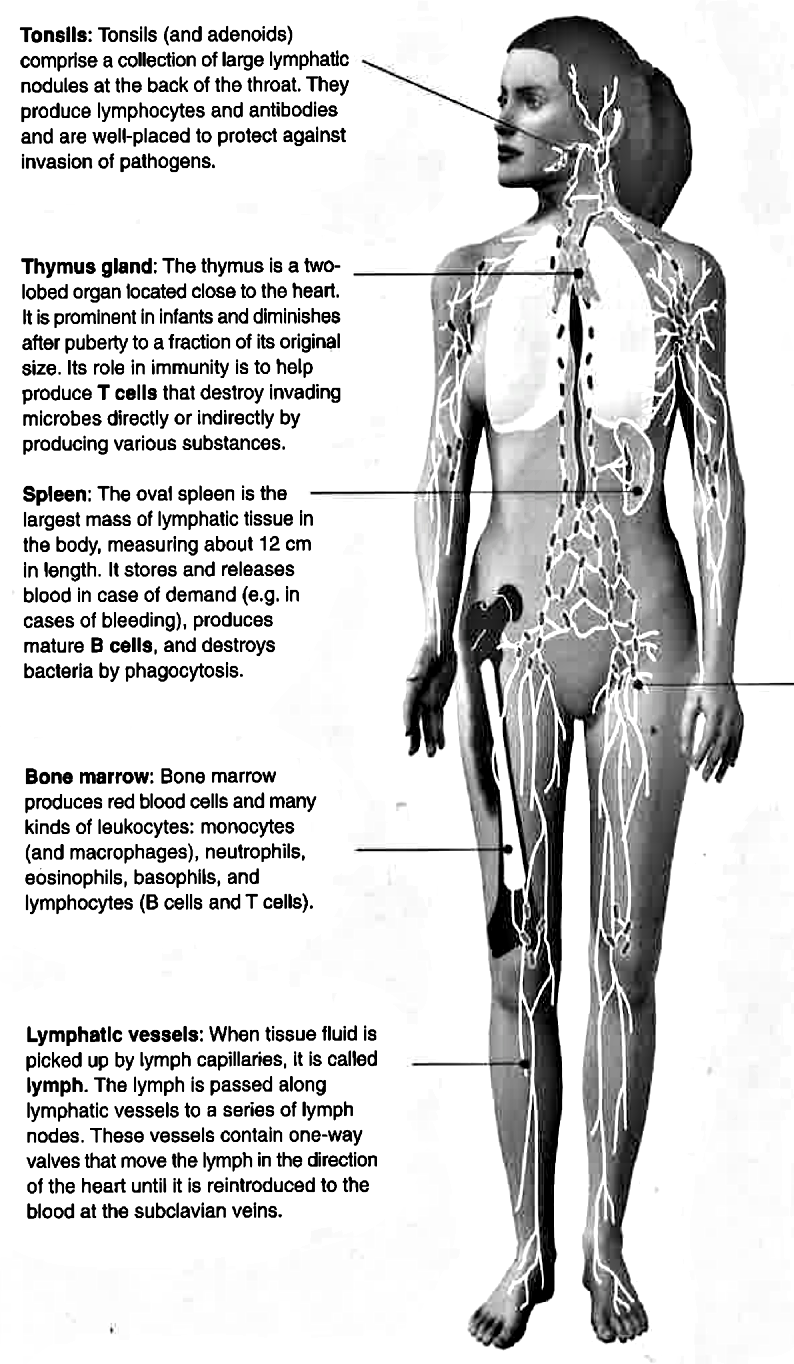
\includegraphics[width=10cm]{/images/biozone-human-0137-1_v1.png}\captionof{figure}[lymph syst from biozone humanbiol p. 137]{The lymphatic system: label the figure according to figure 33.21 (Starr 9ed) in your textbook}  	\label{fig:LymphSystOverv}
	\end{minipage}
	}{%%
	\begin{minipage}[htbp]{12cm}
	\includegraphics[width=10cm]{/images/biozone-human-0137-1_v2.png}\captionof{figure}[lymph syst from biozone humanbiol p. 137]{The lymphatic system: label the figure according to figure 33.21 (Starr 9ed)}  	\label{fig:LymphSystOverv}
	\end{minipage}
	}



\clearpage
\subsection{Three lines of defence}\label{sec:ThreeLinesDefence}
				\begin{mdframed}[style=exampledefault, userdefinedwidth=12cm,frametitle={Starr chapter 34.1}\label{mat:BEISPIELMATERIAL}]
			Our body is warm, wet and full of delicious nutrients - a feast for every microorganism!
			Under the title \textit{What is immunity} you can find a conceptual introduction to the way our body fights off pathogens.
		\end{mdframed}

%  We learned from human history different solutions in this situation: you either fully protect your wealth - you will have to start an arms race (\textit{"'Wettrüsten"', see the cold war}) or rule and divide (\textit{"`herrsche und teile"`, as during the colonial time}). You never can be sure to protect your goods and eventually you get sick and finally you will die, getting rotten by microorganisms.



The arms race against "`bad"' microorganisms is lined up in three lines of defence:

	\begin{enumerate}[itemsep=1.5em, leftmargin=*]
	\item   Match the following terms with the corresponding line of defence:  \textsc{
	adaptive immunity; mechanical barrier; innate immunity; phagocytic white blood cells; lymphocytes, cellular response, chemical barrier; inflammatory response; secretion of mucus; antibodies; antimicrobial proteins; skin; complement proteins}.

	\item Explain which of these three lines are \textbf{unspecific}, which are \textbf{specific} against \textsc{certain germs}!
	\end{enumerate}
%
				\Loesung{\marginline{\href{/share/SB_Unterricht/Biology/hum11_immunobiology/Immune_ Biology_HS16.ppt}{link to ppt ``immunity''}}}{0cm}

% % 	\begin{addmargin*}[-.5cm]{-1.5cm}
	\hspace{-3.6cm}
	 \begin{minipage}{16cm}
		\setlength{\extrarowheight}{6pt}
		 \captionof{table}{Characteristics of the three lines of defence}
		  \vspace{12pt}
		    \begin{tabularx}{16cm}[]{p{5cm} p{5cm} p{6cm}} %
		\toprule
		First line of defence & Second line of defence  & Third line of defence \\\midrule
		 \gap{mechanical barrier}   &  \gap{phagoc. white blood cells} &  \gap{adaptive immunity}\\
		 \gap{chemical barrier}   & \gap{inflammatory response}  & \gap{lymphocytes} \\
		 \gap{secretion of mucus}   &  \gap{complement proteins} & \gap{cellular response} \\
		 \gap{skin}   & \gap{innate immunity}  & \gap{antibodies} \\
		 \gap{antimicrobial proteins} &  &  \\
		\bottomrule
		\end{tabularx}%
		  \label{tab:ThreeLinesDefence}%
	\end{minipage}
% % 	\end{addmargin*}


% \Ersatz{\vspace{0cm}\enlargethispage{2cm} }{\vspace{1cm}}
% \Ersatz{\hspace{-1cm}}{\hspace{-1cm}}

	\vspace{1cm}
	\begin{enumerate}[resume,itemsep=4pt, leftmargin=0cm]
	\item  Use \ding{229} Starr chapter 34 to assist you filling in the cross word (\autoref{fig:CrissCrossBodyDefense})
	\end{enumerate}

	\enlargethispage{2cm}
	\hspace{-3.6cm}
	\begin{minipage}{16cm}
			\begin{multicols}{2}
			\bgroup \Ersatz{\tiny}{\small}
			1. an organism's capacity to resist and combat an infection
				\Loesung{\\ immunity}{0cm}

			2. which underlying process developed the concept of self and non-self?
				\Loesung{\\ evolution}{0cm}

			3. abbreviation for non-self cues
				\Loesung{\\ pamp}{0cm}

			4. set of proteins that can destroy invading cells
				\Loesung{\\ complement}{0cm}

			5. a fast general defence against infection
				\Loesung{\\ innate immunity}{0cm}

			6. what stands the abbreviation 'PAMP' for?
				\Loesung{\\ pathogen associated molecular patterns}{0cm}

			7. a tailored immune defense
				\Loesung{\\ adaptive immunity}{0cm}

			8. cells that mount a quick secondary response even years after a first infection with a specific antigen
				\Loesung{\\ memory cells}{0cm}

			9. physical, chemical and mechanical barriers against invaders are called the [...] of defense
				\Loesung{\\ first line)}{0cm}

			10. a cell that moves around and engulfs ('eats') other cells is ...
				\Loesung{\\ phagocytic}{0cm}

			11. general term for substances which allow partners of the immune system to communicate
				\Loesung{\\ cytokines}{0cm}

			12. The most abundant phagocytic cells are
				\Loesung{\\ neutrophiles}{0cm}

			13. interleukins and interferons are
				\Loesung{\\ cytokines}{0cm}

			14. Cells of the innate immune system which alert the adaptive immune system
				\Loesung{\\ cendritic cells}{0cm}

			15. Eosinophiles contain vesicles filled with destructive enzymes targeting
				\Loesung{\\ parasites}{0cm}

			16. The nervous system may cause degranulation of
				\Loesung{\\ mast cells}{0cm}

			17. Cell of the adaptive immune system, recognizing a specific antigen:
				\Loesung{\\ lymphocyte}{0cm}

			18. an infected cell may be destroyed by a
				\Loesung{\\ cytotoxic t-cell}{0cm}

			19. a cancerous (von Krebs befallen) cell may be destroyed by a
				\Loesung{\\ natural killer cell}{0cm}

			20. approximative number of different antigens detected by the innate immune system
				\Loesung{\\ thousand}{0cm}

			21. approx. response time for the adaptive immune system - in 'days'
				\Loesung{\\ seven}{0cm}
			 \egroup
	\end{multicols}
	\end{minipage}

%
% 	\vspace{4pt}
% 	\hspace{1cm}
	 \areaset[0cm]{20cm}{28cm}
	\thispagestyle{empty}
	\Ersatz{
		\begin{minipage}[htbp]{22cm}
		\centering {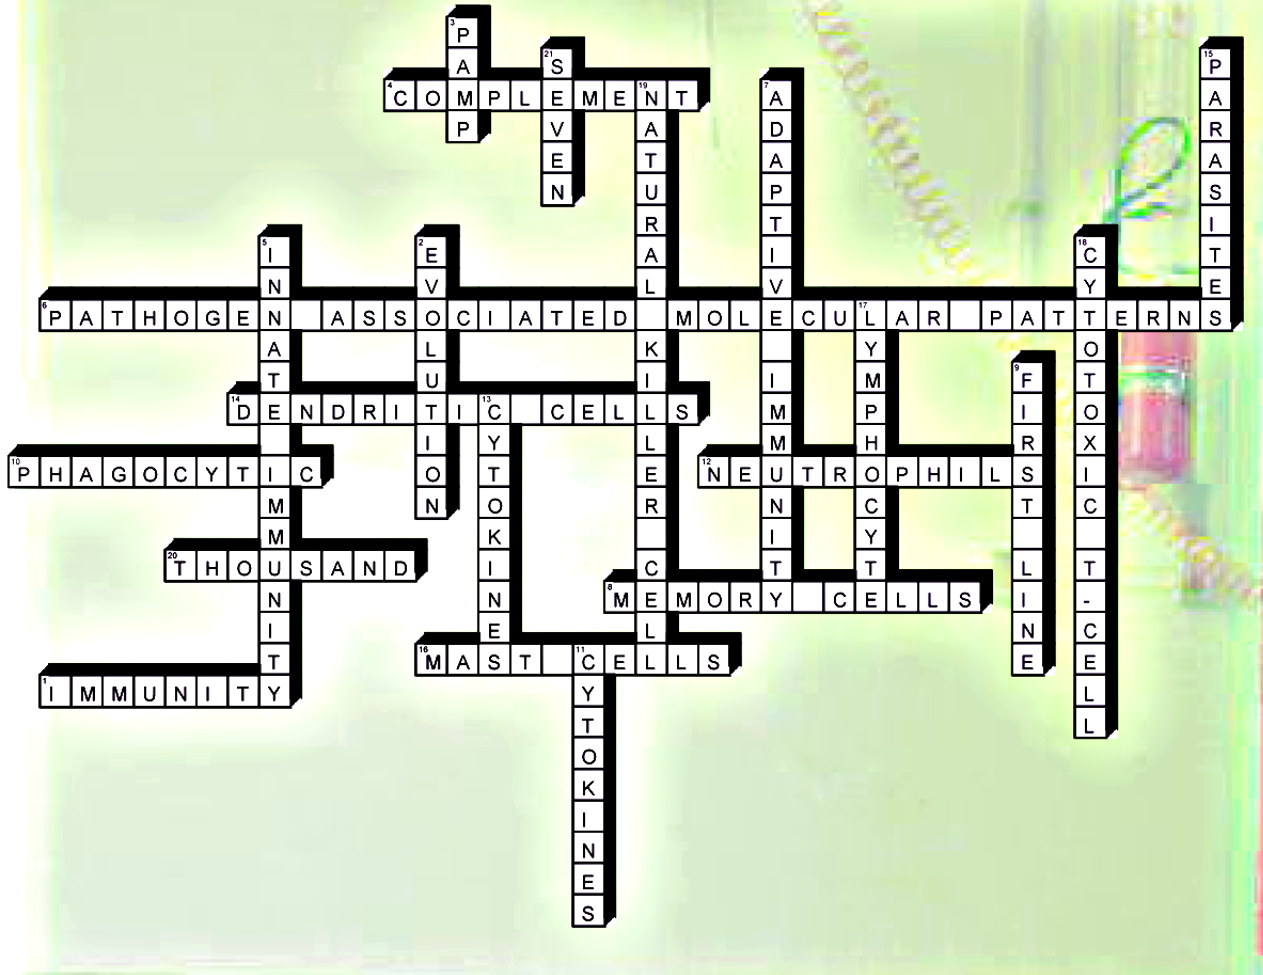
\includegraphics[width=1\textwidth,angle=90]{/share/SB_Unterricht/Biology/hum11_immunobiology/BodyDefence-CrissCross_L_v2.png}} \captionof{figure}[VERZEICHNISEINTRAG]{Crossword on immune response - introduction}  	\label{fig:CrissCrossBodyDefense}
		\vspace{2pt}
		\end{minipage}
		}%
		{
		\begin{minipage}[htbp]{20cm}
		\centering {\includegraphics[width=1\textwidth]{/share/SB_Unterricht/Biology/hum11_immunobiology/BodyDefence-CrissCross_S_v3}} \captionof{figure}[VERZEICHNISEINTRAG]{Crossword on immune response - introduction}  	\label{fig:CrissCrossBodyDefense}
		\vspace{2pt}
		\end{minipage}
		}%


 \areaset[0cm]{15cm}{27.4cm}
\subsection{How cells recognise each another and form tissues}
\Pointinghand\, May cells erronously stick to the wrong partner? The following figures  (\textit{taken vorm Markl, chp 3.2}) give you an answer:

\begin{enumerate}[itemsep=1.5em, leftmargin=*]
\item  The cells of two differently colored sponges (\textit{yes, these are living organisms!}) of the same species were isolated through a sieve and then mixed up. Describe the outcome of this experiment and draw a general conclusion!
\end{enumerate}
			\vspace{1.4cm}
			\begin{figure}[htp]\centering
		  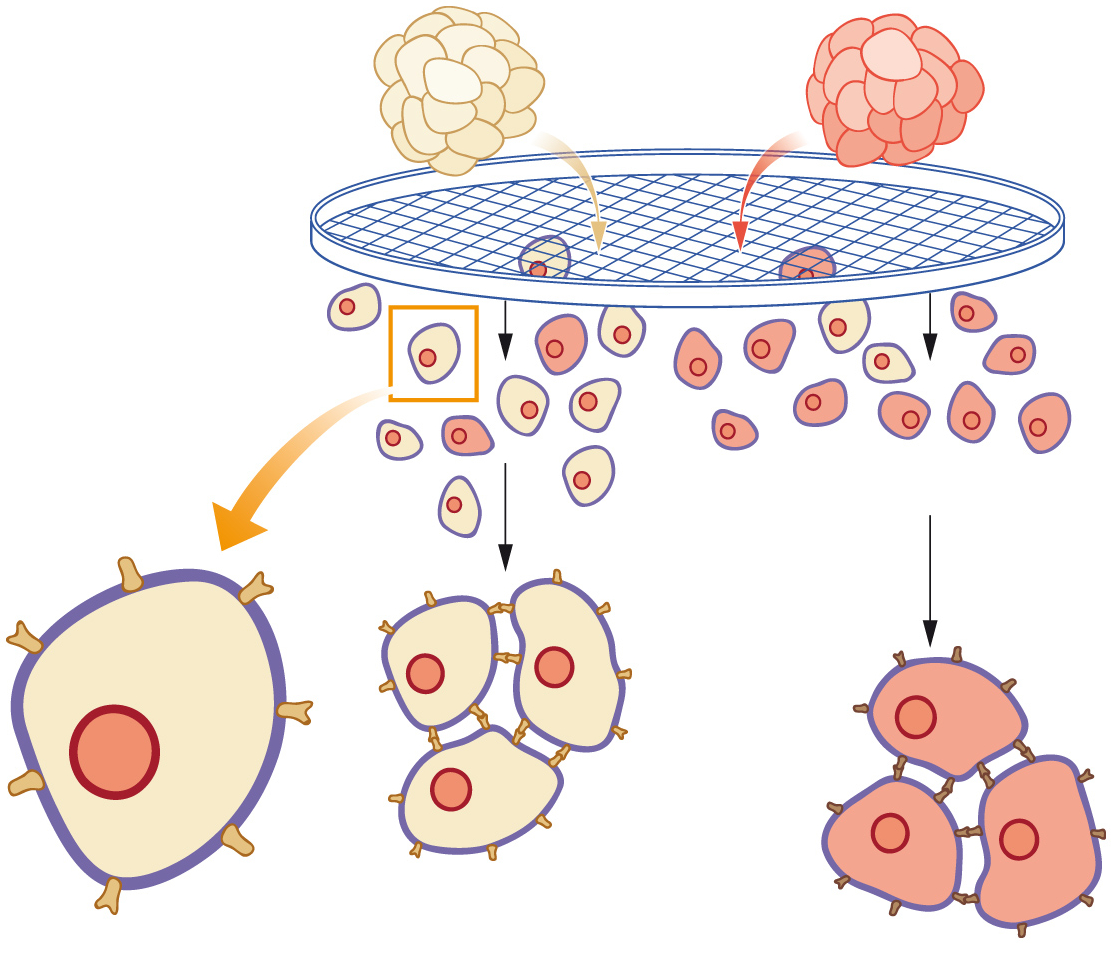
\includegraphics[width=0.5\textwidth]{/share/00_SCHULE_DATA-add/bilder_saz/Markl_Bilder/1_4_Zellen/3_Biomembranen_und_Transportvorgaenge/03_02_01_1.jpg}
		  \caption[Schwammzellen finden sich aus Markl 3.2]{Cells of two different sponges were experimentally mixed (coloured figure in Markl 3.2 or on \ding{253} \textsc{Moodle}).}
		  \label{fig:SchwammZellen}
		%\setfloatalignment{b}
		\end{figure}

			\begin{figure}[htp] \centering
		  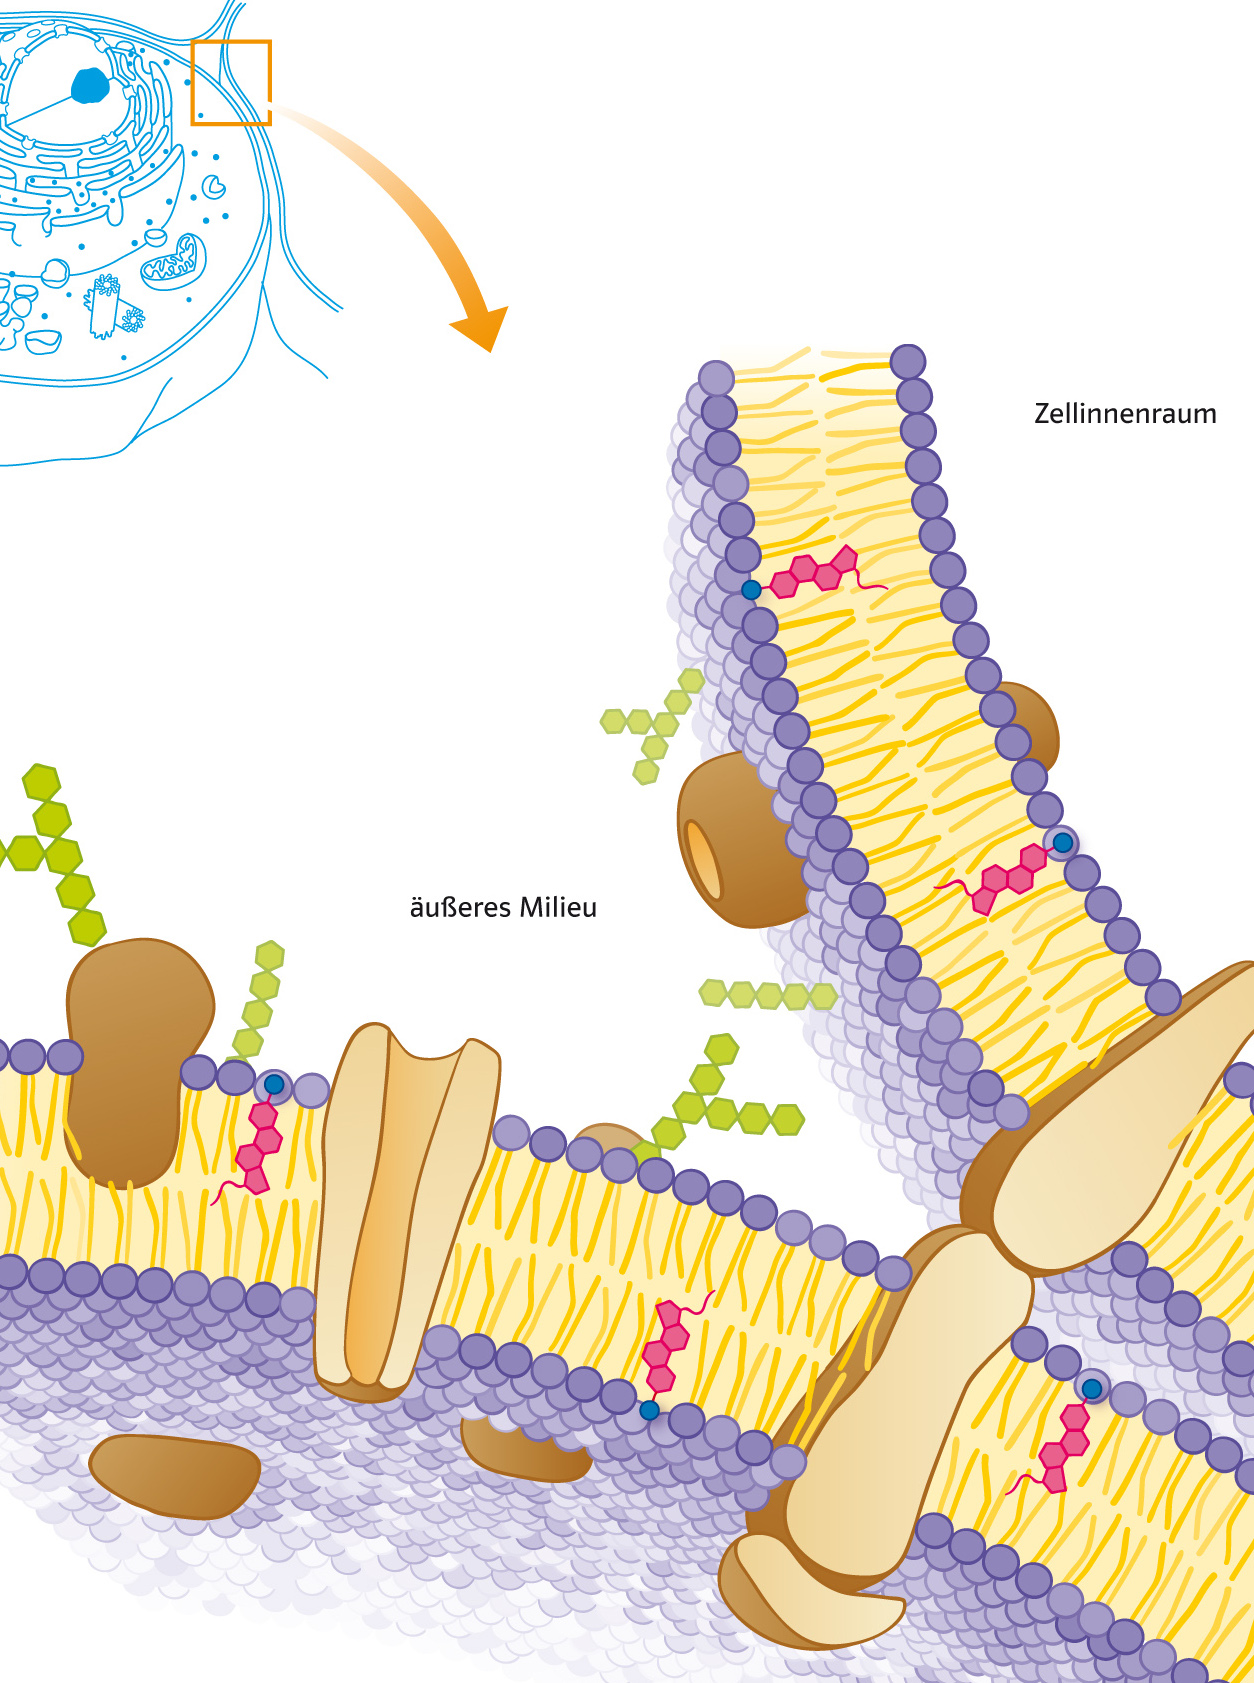
\includegraphics[width=0.5\textwidth]{/share/00_SCHULE_DATA-add/bilder_saz/Markl_Bilder/1_4_Zellen/3_Biomembranen_und_Transportvorgaenge/03_01_01_1_v1.jpg}
		  \caption[Aufbau Zellmembran aus Markl 3.1]{Fluid mosaic model of cell membranes (coloured figure in Starr (9ed) 4.3 or on \ding{253} \textsc{Moodle})}
		  \label{fig:ZellmembraneGlykolipide}
		%\setfloatalignment{b}
		\end{figure}

\clearpage
\subsection{The family tree of blood cells}
\Pointinghand\, Knowing the "`who is who"' in the family of blood cells tells us what they may have in common and how they are related to each other:

\hspace{-3cm}
    \begin{figure}[htbp]
    \begin{minipage}{7cm}

      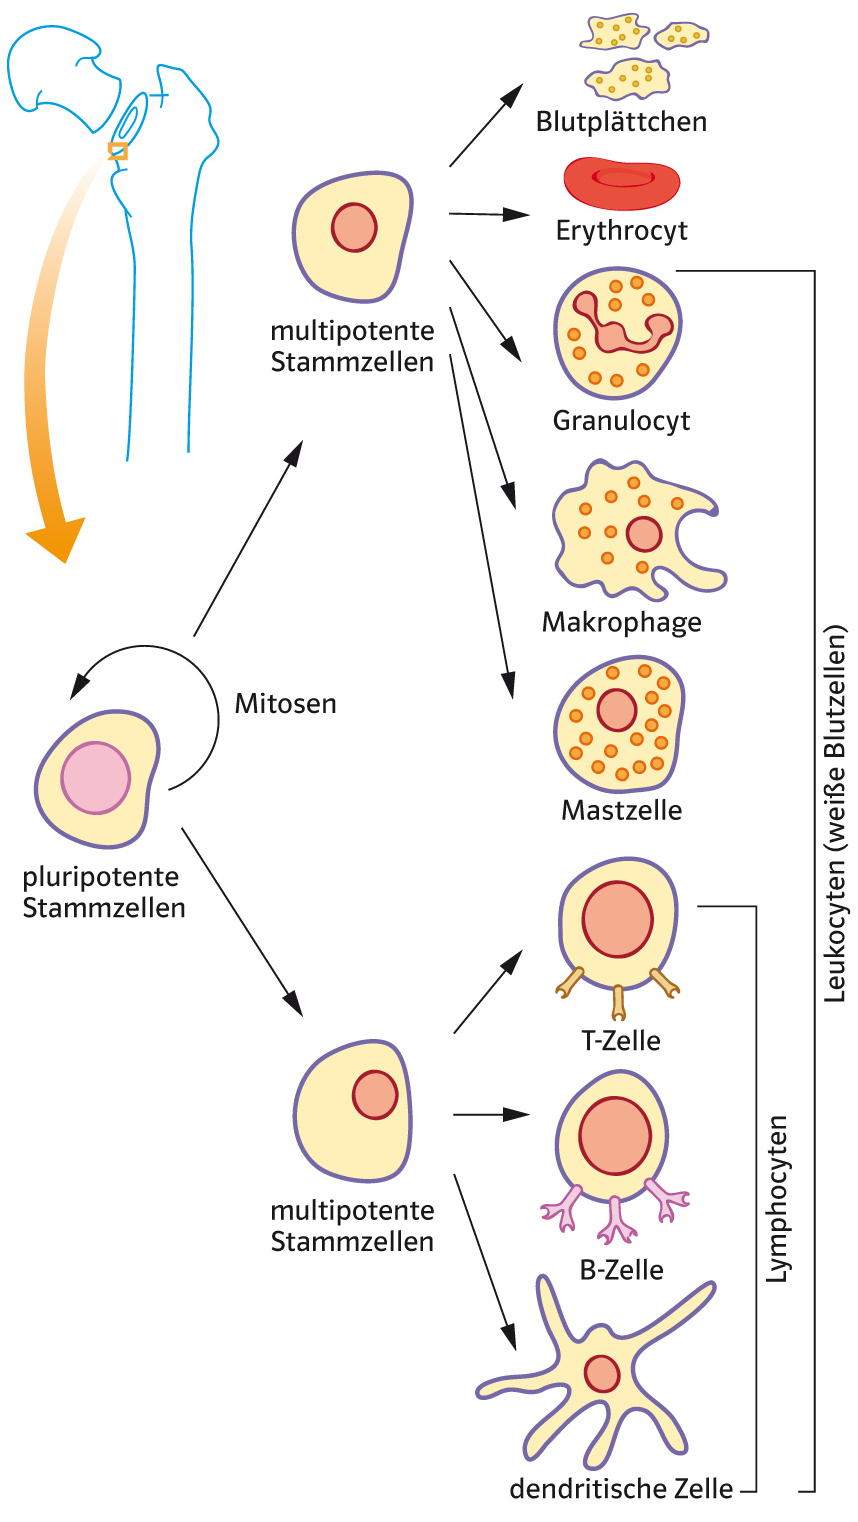
\includegraphics[width=0.8\textwidth]{/share/00_SCHULE_DATA-add/bilder_saz/Markl_Bilder/9_16_Genetik/13_Entwicklungsgenetik/13_04_01_0.jpg}
      \caption{The various blood cells stem from multi-potent stem cells. (\textit{figure taken from Markl, 13.4}) }  \label{fig:BlutGenese}
    \end{minipage}\hfill
    \begin{minipage}{9cm}
     \hfill
      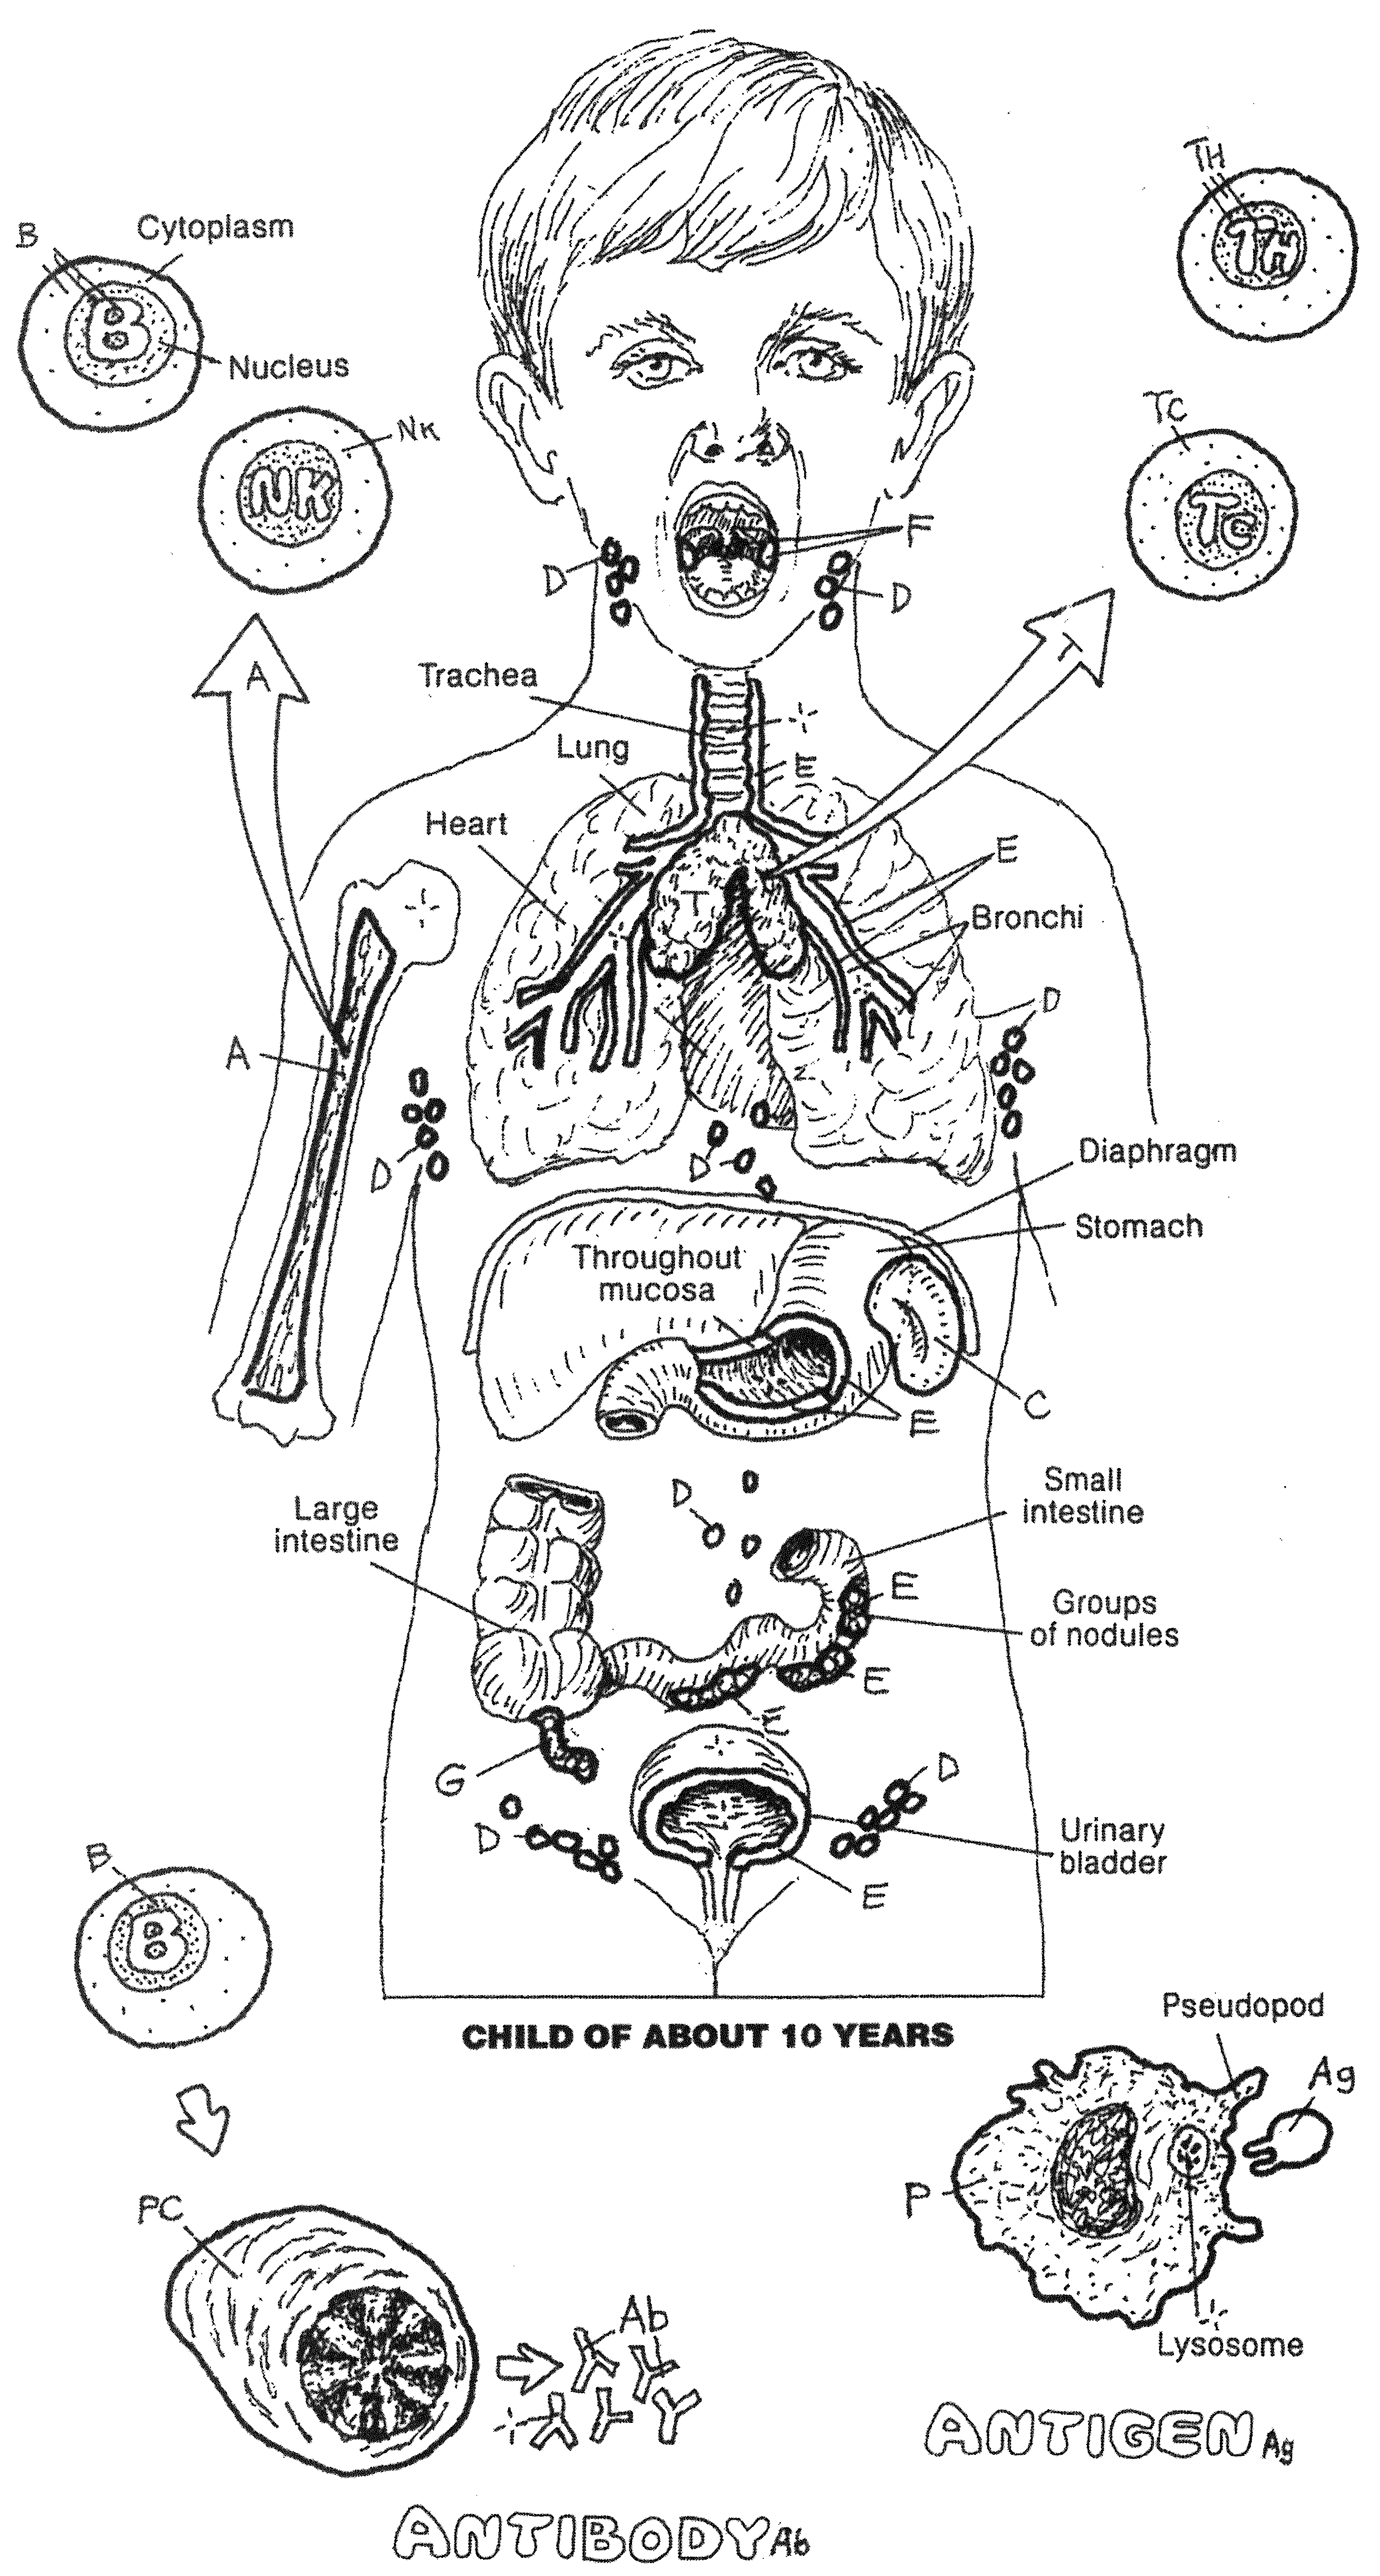
\includegraphics[width=0.8\textwidth]{/share/00_SCHULE_DATA-add/bilder_saz/Humanbio_Bilder/Anatomie_MalAtlas_en/AnatomyCol-121_v1.png}
      \caption{White blood cells need to be trained for their job (\textit{from Markl Kap. 16.1.}) \textbf{A} Bone Marrow; \textbf{T} Thymus; \textbf{C} Spleen; \textbf{D} Lymph node; \textbf{E} lymphatic tissue connected to the intestines; \textbf{F} Tonsils; \textbf{G} Appendix; \textbf{B} B-Lymphocytes; \textbf{PC} Plasma-Cell; \textbf{TH} T-Helper-Cell; \textbf{TC} T-Cytotoxic-Cell; \textbf{NK} Natural Killer Cell; \textbf{P} Phagocyte
      }  \label{fig:LymphOrgane}
    \end{minipage}
	 \end{figure}



\Lehrer{ \vspace{2cm}
		Diskussion des Konzepts Stammzelle\\
		Einführen der Typen von weissen B.K.\\
		Bildungs- und Ausbildungs-Orte der weissen B.K.
		}

\clearpage \enlargethispage{1.8cm}
\subsection{Discrimination of self and foreign}
\Pointinghand\, This chapter explains how our immune system discriminates self from foreign - a prerequisite to any action against pathogens.

\subsubsection{The Major Histocompatibility Complex One (MHC-I) acts as the cells' identity card}
\begin{mdframed}[style=RedGray]
\textbf{ 1.} NO infection present: "`safe"' and healthy every day life of cell.
\end{mdframed}


% \begin{mdframed}[style=RedGray]
	\begin{minipage}{14cm}
	 \centering
		\includegraphics[width=1\textwidth]{/share/00_SCHULE_DATA-add/bilder_saz/Humanbio_Bilder/humanbio_Tortora-en/ch22/pap14_fig_22_14.jpg}
	\end{minipage}
% 	\end{mdframed}
\vspace{2cm}

%
% 	\setlength{\extrarowheight}{4pt}
% 	\begin{tabularx}{14cm}[]{>{\textbf}m{0.7cm} >{\textsc}m{3cm} X} \toprule
% 	\textbf{Nr} &  \textbf{Prozess} \\ \midrule
% 	1 &  Lysosom  & Abbau von zelleigenen Proteinen in Peptidfragmente \\
% 	2 & Endopl. Retic. (ER) & Synthese von MHC Molekülen in ein Vesikel  \\
% 	3 & Golgi-Vesikel & Vesikel mit MHC-I nimmt Peptid (Proteinbruchstücke) auf und wird zum MHC-Vesikel \\
% 	4 & MHC-Vesikel &  Peptide werden an MHC-I gebunden und wandert zur Zellmembran \\
% 	5 & Zellmembran & Exocytose des mit Peptid beladenen MHC-I Komplexes und Einbau in die Zellmembran \\
% 	6 & Zellmembran & tausende von MHC-I Komplexe über der ganzen Zelloberfläche zeigen laufend die typischen zelleigenen Proteine \\
% 	\bottomrule
% \end{tabularx}

\vfill \bgroup \centering
\Pointinghand\, The cells of the immune system permanently scan the surface of every body cell. As long as the immune system encounters well known protein-fragments posted on MHC-I the cell is considered healthy and the immune system won't get activated. \egroup
\vfill

\clearpage
\subsubsection{In case of an infection, MHC-I triggers the "`alarm"'}
\vspace{0.2cm}
\begin{mdframed}[style=RedGray] \textbf{2.} An infection (or a tumor) is present: this means "`sickness"' to any kind of cells. \end{mdframed}

% \Kommentar{
% \begin{mdframed}[style=RedGray]
	\begin{minipage}{16cm}
	 \centering \vspace{0.4cm}
		\includegraphics[width=0.7\textwidth]{/share/00_SCHULE_DATA-add/bilder_saz/Humanbio_Bilder/humanbio_Tortora-en/ch22/pap14_fig_22_14.jpg}
	\end{minipage}
	% 	\end{mdframed}
	\vspace{0.2cm} This is the \textsc{same} figure as on the previous page \textsc{but} DIFFERENT proteins are shown: fragments of either a \textbf{virus} or distorted proteins e.g. typical for \textbf{cancer}.
% 		}{}{5cm}{}

\vspace{0.3cm}
\bgroup \centering \Pointinghand\, Whenever a cell presents unusual proteins such as virus fragments or proteins that derive from a mutation within the cell's genome on its MHC-1 flag poles the immune system sets the alarm! This starts the immune response to fight off every cell that shows the same type of antigen (\textit{"`strange or foreign protein"'})!
\egroup

\enlargethispage{1.4cm}
\vfill
	\hfill	\begin{mdframed}[style=exampledefault,leftmargin=-1cm, userdefinedwidth=16cm,frametitle={\hfill Antigene: "`antibody generating agent"'\hfill}\label{mat:BEISPIELMATERIAL}]
			Every structure which causes the formation of antibodies is called an \textsc{antigen}. Examples are the surface proteins of erythrocytes (see the \textsc{AB0}-blood-system) OR strange proteinfragments shown on MHC-1 (\textit{this chapter}) OR surface structures of pathogens (see fig.\ref{fig:AntigeneEpitopeAntikoerper}) OR surface structures various kind of foreign matter such as pollen (hay fever).\\
			\emph{note} the difference between  \emph{antigen} and \emph{epitop} as shown here:

	 \centering
		  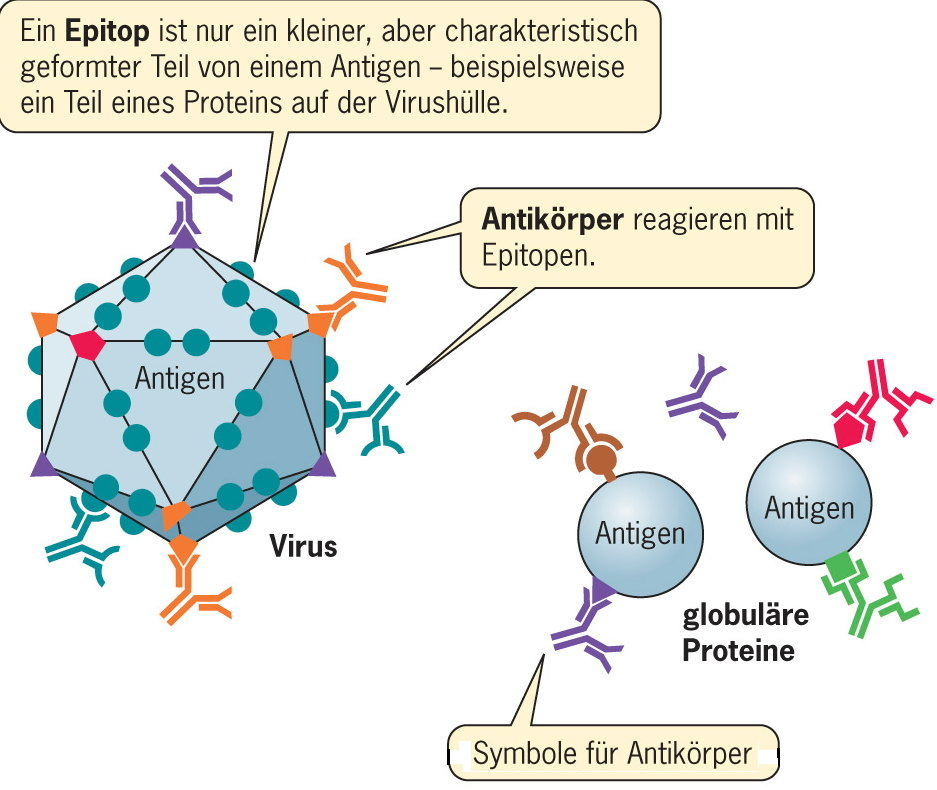
\includegraphics[width=0.5\textwidth]{/share/00_SCHULE_DATA-add/bilder_saz/Purves/abbildungen/kap-18/18-06_v2.jpg}
		  \captionof{figure}[Antigene, Epitope, Antikörper; aus Purves, 7. Aufl. 2006, Abb. 18-06]{An \textbf{epitop} is a specific part of an antigen which causes the formation of a specific antibody (see  \ding{229} Starr ... }
		  \label{fig:AntigeneEpitopeAntikoerper}
		\end{mdframed}
% \vspace{1cm}

\clearpage
\subsection{Phagocytosis, cells of the immune system and MHC-II}
\Pointinghand\, Cells of the immune system are capable of \textsc{phagocytisis}, i.e. to ingest and digest foreign cells and other particles. Fragments of the eaten up foreign material is presented attached to "`Major Histocompatibility Complexes Two"` (MHC-II) on the outer membrane of \textsc{antigen presenting cells}:

\vspace{1cm}
% \Kommentar{
% \begin{mdframed}[style=RedGray]
	\begin{minipage}{12cm}
	 \centering
		\includegraphics[width=1\textwidth]{/share/00_SCHULE_DATA-add/bilder_saz/Humanbio_Bilder/humanbio_Tortora-en/ch22/pap14_fig_22_13.jpg}
	\end{minipage}
% 	\end{mdframed} \vspace{0.2cm}
% 		}{}{6cm}{}

% 	\setlength{\extrarowheight}{4pt}
% 	\begin{tabularx}{14cm}[]{>{\textbf}m{0.7cm} >{\textsc}m{3cm} X} \toprule
% 	\textbf{Nr} &  \textbf{Prozess} \\ \midrule
% 	1 & Zellmembran & Phagocytose (\textit{Zellfressen}) eines Antigens \\
% 	2 & Phagosom (Vesikel) & Verdau des Antigens in Peptidfragmente \\
% 	3 & Endopl. Retic. (ER) & Synthese von MHC Molekülen und Verpackung in ein Vesikel  \\
% 	4 & Vesikel & Verschmelzung von  Phagosom und MHC-Vesikel  \\
% 	5 & MHC-Vesikel & Antigen-Peptidfragmente binden an MHC-II Moleküle \\
% 	6 & Zellmembrane & Die MHC-II Komplexe zeigen die fremden Proteine (Peptid-Fragmente) auf der Zelloberfläche. Das ist eine Alarmglocke! \\
% 	\bottomrule
% \end{tabularx}


\vfill
		\begin{mdframed}[style=exampledefault,leftmargin=2cm userdefinedwidth=14cm,frametitle={MHC-I, MHC-II and Interleukins allow to trigger a immune reaction }\label{mat:BEISPIELMATERIAL}]
			Aberrant material (antigens) presented both on MHC-I and / or MHC-II triggers the communication among cells of the immune system. In response the cells of the immune system produce signalling chemicals, referred to \textsc{cytokines} or more specific to \textsc{interleukins}

			\centering Communication among cells is crucial at the interface of \textsc{unspecific} and \textsc{specific} immune response as well as in the coordination and control of the highly complex specific immune response.
		\end{mdframed}
	\vspace{1cm}



\clearpage \enlargethispage{1.6cm}
\subsection{Antibodies and Receptors}
\Pointinghand\,\, Both secreted antibodies \emph{freely moving in blood and lymph} and receptors \emph{membrane bound antibodies} are the counter players of antigens - they do recognise them. You already well know the antibodies of the $AB0$-blood group system, that match the respective antigens. Lets now have a closer look:


		\begin{minipage}{9cm}
		  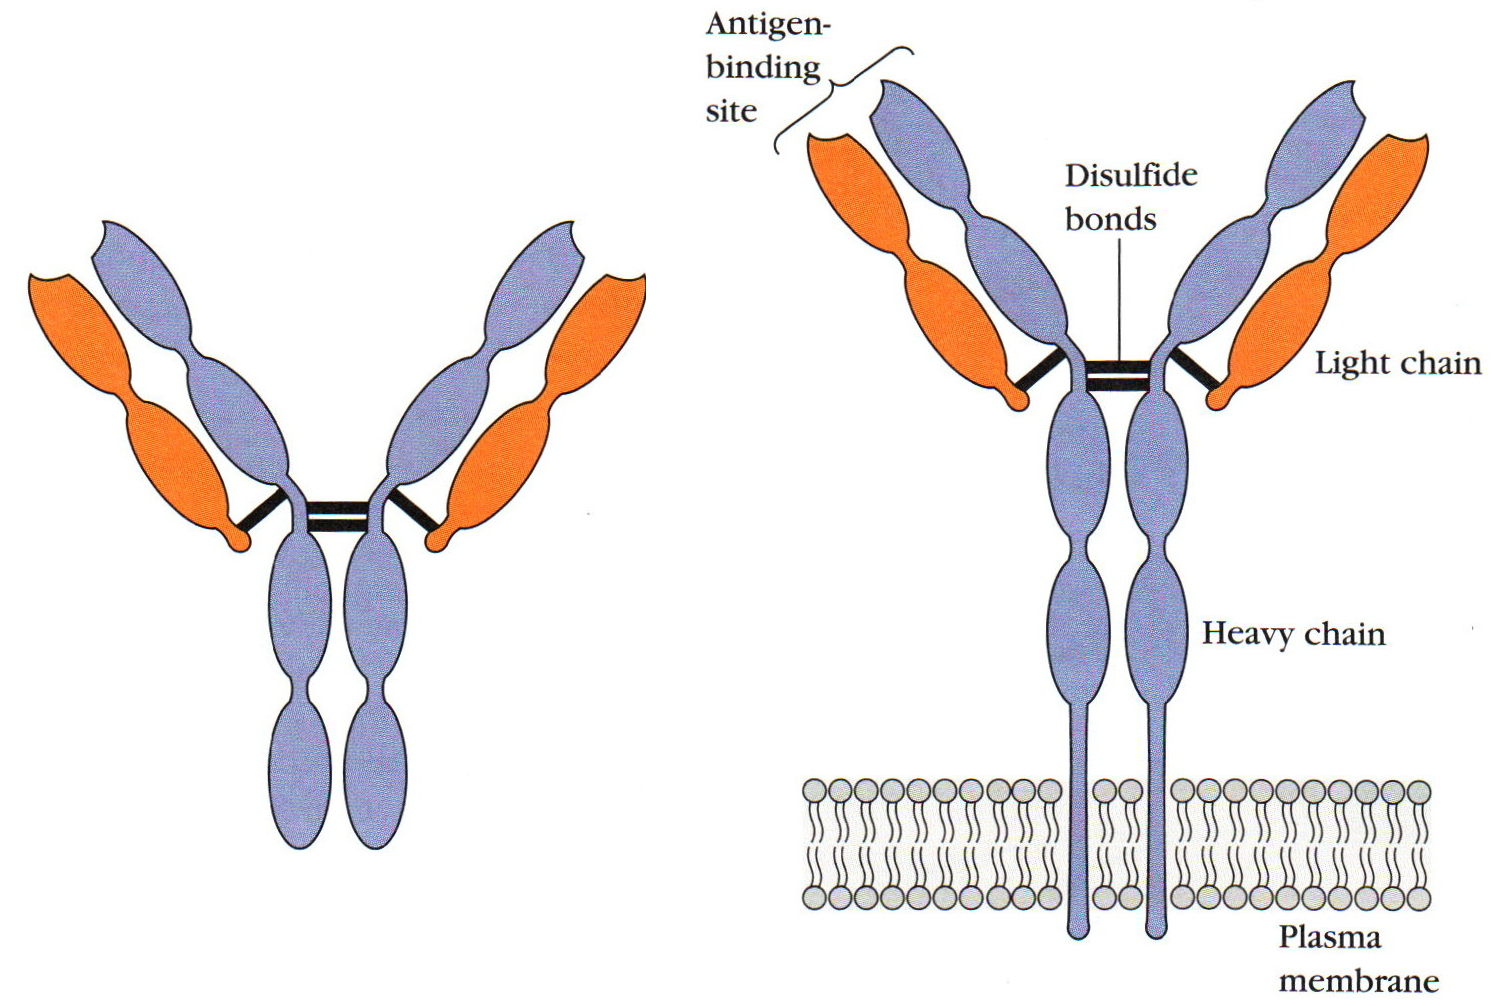
\includegraphics[width=0.9\textwidth]{/share/SB_Unterricht/Biologie/hum11_Immunbiologie/Antikoerper-Rezeptor_Kuby-Fig-01-07_v2.jpg}
		  \captionof{figure}[B-Rezeptor und B Antikörper aus Kuby 8th ed. p. 12 (Fig. 1-7)]{Model of a free moving (secreted) antibody (left) and a receptor attached to the membrane (right)  \textit{source: Kuby, 8th ed.} More details in  \ding{229} Starr (9ed) 34.4 }
		  \label{fig:RezeptorAntikoerper}
		\end{minipage}
% 		\hspace{0.4cm}
		\begin{minipage}{6cm}
		 \includegraphics[width=1\textwidth]{/share/SB_Unterricht/Biologie/hum11_Immunbiologie/Toll-Rezeptor_Kuby-Fig-03-010_v2.jpg}
		  \captionof{figure}[Toll-Rezeptor aus Kuby 8th ed p. 63 (Fig. 3-10)]{Toll receptor of a macrophage - this receptor matches with typical glykolipids (or glykoproteins) on the surface of bacteria \textit{Quelle: Kuby, 8th ed.}}
		  \label{fig:TollRezptor}
		\end{minipage}

		\begin{mdframed}[style=exampledefault, userdefinedwidth=16cm,frametitle={Toll-receptors, Immunoglobulines, cell-bound Receptors }\label{mat:BEISPIELMATERIAL}]
			\begin{itemize}
				\item Toll Receptors are found on the surface of macrophages and they are crucial in the \textsc{innate} immune response.

				\item Toll receptors recognise typical surface antigens ($\rightarrow$~ "' \textit{unspecific response"`}) of most bacteria and allow macrophages to immediately phagocyte the bacteria.

				\item Immunoglobulines (Ig) are the typical kind of secreted antibodies and they are crucial in the \textsc{adaptive immune response}.

				\item Membrane-bound receptors of the \textsc{lymphocytes} recognise antigens attached to either  MHC-I or MHC-II.

				\item Every type of immunglobuline (Ig) or membrane-bound-receptor can identify a single type of antigen.

				\item Because their are billions of different antibodies (Ig or receptors) one will always match to a new kind of antigen!
			\end{itemize}
		\end{mdframed}





		\begin{minipage}{15.5cm}\centering
		  \includegraphics[width=0.9\textwidth]{/share/SB_Unterricht/Biologie/hum11_Immunbiologie/Ecoli-Lipopolysaccharide_Kuby-Fig-03-09_v1.png}
		  \captionof{figure}[E. coli Zellwand aus Kuby 8th ed p. 63 (Fig. 3-9)]{Darstellung der Zellwand eines \textit{E. coli} (Darm-)Bakteriums: Die Lipopolysaccharide auf der Aussenseite werden (in der Regel) von den Toll-Rezeptoren der Makrophagen erkannt und lösen die \textsc{unspezifische} Immunreaktion aus. \textit{Quelle: Kuby, 8th ed.}}
		  \label{fig:BakterienZellwand}
		\end{minipage}

% \areaset[0cm]{11.5cm}{27.4cm}
\subsection{Innate immunity - your second line of defence}\label{sec:ImmuneInnate}\label{ssc:ImmuneInnate}
Work with your textbook \ding{229} chapter 34.4 (Starr 9ed 34.3).

		\begin{mdframed}[style=exampledefault, userdefinedwidth=12cm,frametitle={Starr chapter 34.3}\label{mat:BEISPIELMATERIAL}]
			Starr explains you which types of cells are capable of phagocytosis. The \emph{complement}-proteins form another part of the innate immune system. The \emph{inflammation} is the ``battle field'' of the innate immune system and \emph{fever} is the recordable outcome of such a kind of immune reaction.
		\end{mdframed}

	\begin{enumerate}[itemsep=1.5em, resume, leftmargin=*]
	\item  Match the terms and explanations in table \ref{tab:InnateImmunityLabels} with the charts in figure \ref{fig:InnateImmunityFigure}!
	\end{enumerate}

% 			\begin{figure}[htp]
				\begin{addmargin*}[-2cm]{-2cm}
	 \begin{minipage}{16cm}
		  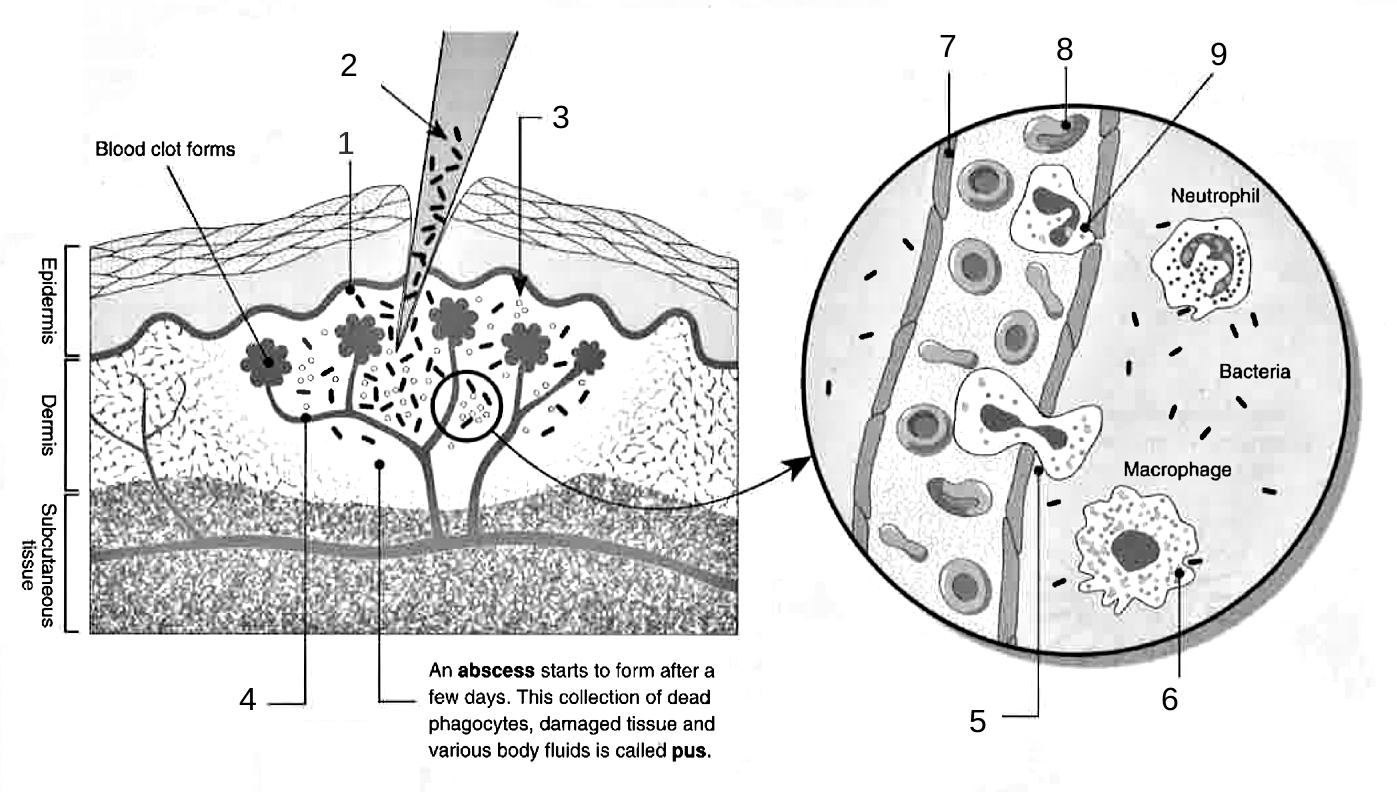
\includegraphics[width=1\textwidth]{/images/biozone-human-0135_v3.png}
		  \captionof{figure}[VERZEICHNISEINTRAG]{The innate immune reaction, synopsis}
		  \label{fig:InnateImmunityFigure}
		%\setfloatalignment{b}
% 		\end{figure}
	 \end{minipage}
				\end{addmargin*}


	\begin{addmargin*}[-2cm]{-2cm}
	 \begin{minipage}{16cm}
% 		 \begin{table}[!htbp]
		\setlength{\extrarowheight}{6pt}
		 \captionof{table}{Text pieces taken from figure \ref{fig:InnateImmunityFigure}}
		  \vspace{12pt}
		    \begin{tabularx}{16cm}[]{X p{2cm}} %
		\toprule
		Structure or function& Legend for figure \ref{fig:InnateImmunityFigure}   \\\midrule
		Bacteria are engulfed and destroyed by phagccytes (macrophages and neutrophils).  & \gap{  6 } \\
		Bacteria entering on knife or other sharp object.   & \gap{  2 } \\
		 Phagocytes stick to capillary walls.  & \gap{ 9  } \\
		 Bacterium  & \gap{  1 } \\
		Blood vessels increase diameter (vasodilatation) and permeability.  & \gap{ 4  } \\
		Capillary wall & \gap{  7 } \\
		Red blood cells & \gap{8   } \\
		Phagocytes squeeze between cells making up blood vessel walls.   & \gap{ 5  } \\
		Chemicals (e.g. histamines and prostaglandins) are released by damaged cells, attracting more and more phagocytes to this infection.   & \gap{ 3  } \\
		\bottomrule
		\end{tabularx}%
		  \label{tab:ThreeLinesDefence}%
% 		\end{table}%
	\end{minipage}
	\end{addmargin*}


\subsubsection{Opsonierung von Krankheitserregern}
\Pointinghand\, Der Wirbeltierkörper produziert Proteine ("'Opsonine"`), welche auf der Oberfläche von Bakterienzellwänden an Oberflächenstrukturen haften, welche es bei vielen Bakterien, aber nicht bei tierischen Zellen gibt. Diese Opsonine wirken für die Fresszellen wie Signalfahnen: "'\textit{Achtung, hierhin und auffressen!}"`. \Forward\, \href{https://cloudfs.tam.ch/share/b57cd0560b90e9f2b2f344aaef286649}{Animationsfilm zur Opsonierung auf  \ding{229} moodle }

\subsubsection{Das Komplementsystem}
\Pointinghand\, Wie bei den Opsoninen, binden die Komplementproteine and Bakterienoberflächen  \ding{229} Markl Kap. 16.2 (ganz am Schluss) und \href{https://cloudfs.tam.ch/share/362f92164b2771f7806ebc86e1db186b}{Animation zum Komplementsystem}


\subsubsection{Fieber unterstützt die Abwehrreaktion}

\begin{enumerate}[itemsep=1.5em, leftmargin=*]
\item  Lesen Sie den nachfolgenden Text übers Fieber - wo nötig setzen Sie ihren Dictionnaire ein! Machen Sie sich passende (Rand-)Notizen!
\end{enumerate}

\begin{minipage}{16cm}
	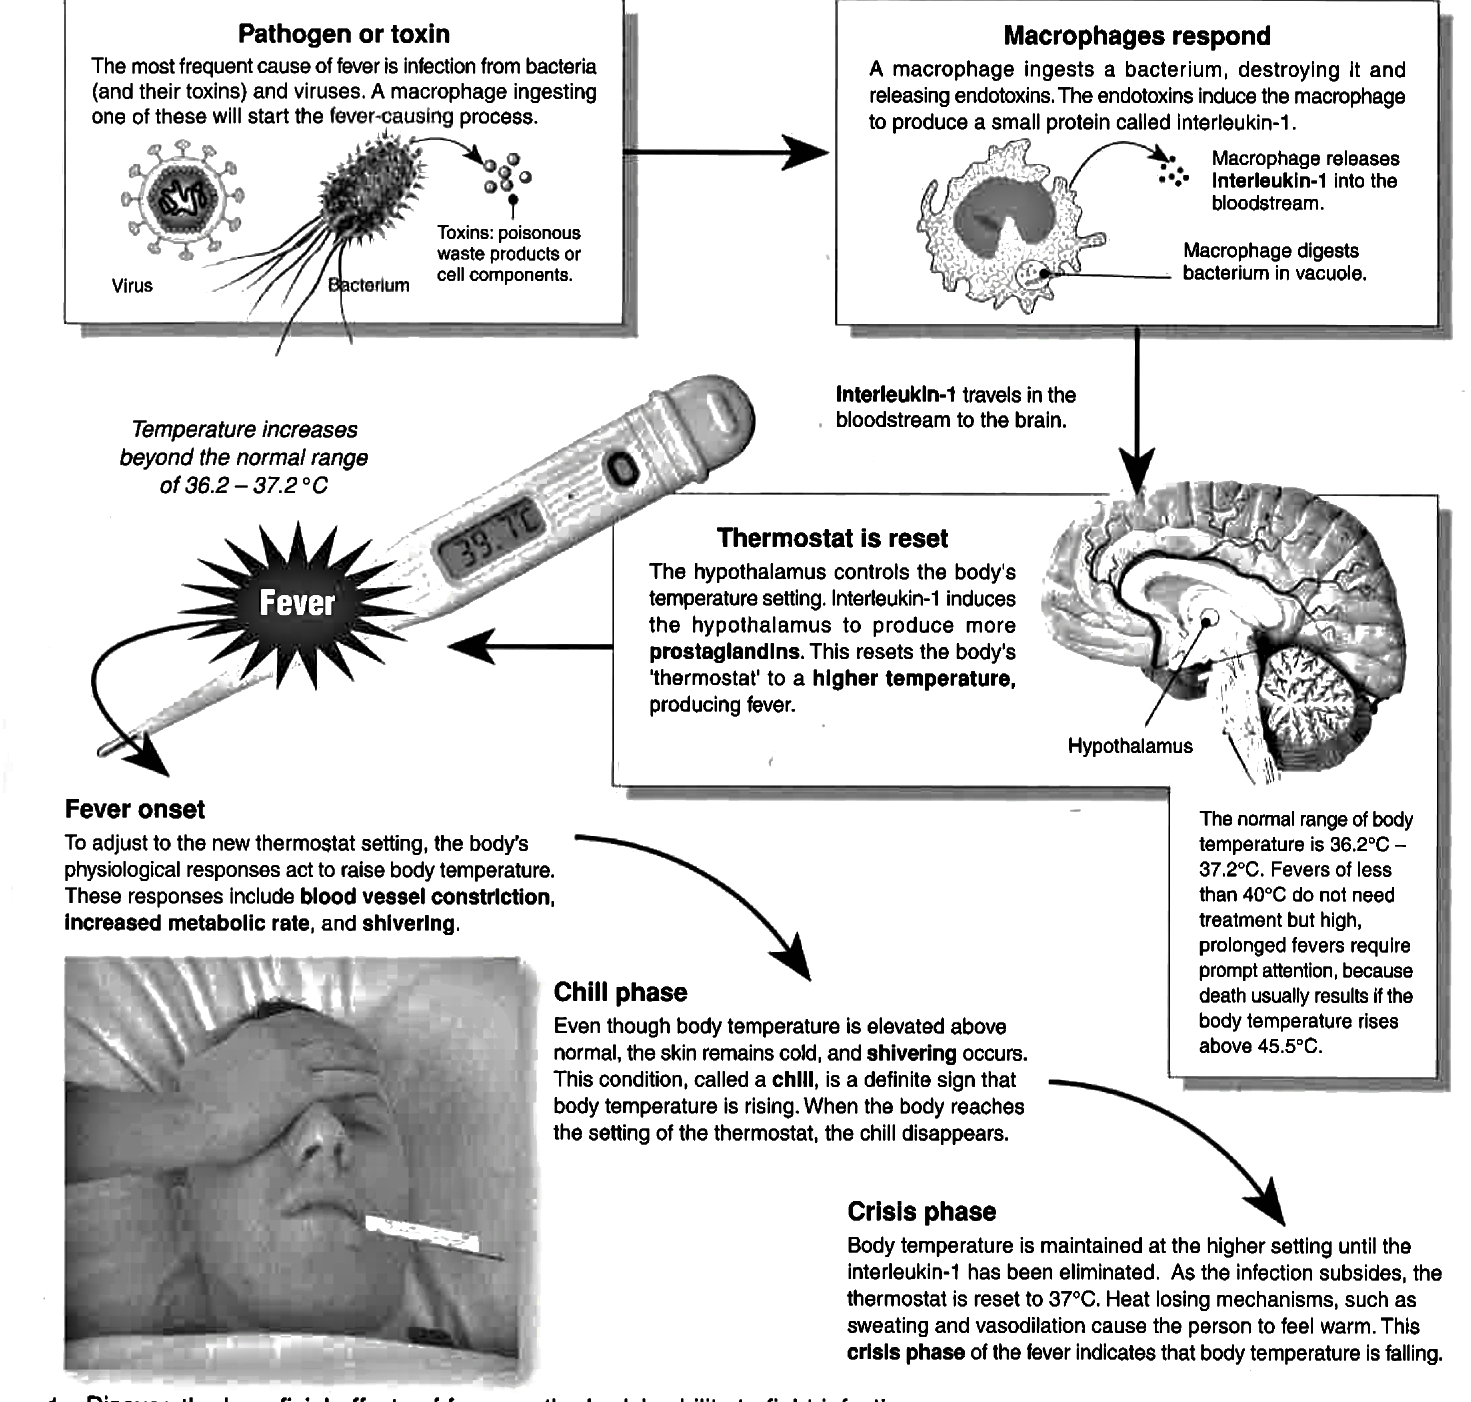
\includegraphics[width=1\textwidth]{/images/biozone-human-0136_v2.jpg}
	 \captionof{figure}[Fieberdarstellung aus Biozone Humans p.136]{Eine erhöhte Körpertemperatur unterstützt die Heilung effizient, denn das Wachstum vieler Bakterien wird gehemmt und metabolische Prozesse laufen rascher ab (Teilchenbewegung, RGT-Regel). Die normale Körpertemperatur liegt bei 36.2 bis 37.2\degreecelsius\, und Temperaturen über 45.5\degreecelsius\, bedeutet Todesgefahr.}
\end{minipage}



\clearpage
\subsection{Adaptive Immune Response (third line of defence)}\label{ssc:AdaptiveImmunity}

		\begin{mdframed}[style=exampledefault, userdefinedwidth=12cm,frametitle={Starr chapter 34.4}\label{mat:BEISPIELMATERIAL}]
			Not the editor's choice this spread, but fine to make you acquainted with the sheer infinite variability of receptors, antigens and antibodies. Read this section carefully and make sure you understand the concepts. However, don't learn by heart the five classes of antibodies (\ding{229} Table 34.3).
		\end{mdframed}

	\begin{enumerate}[resume, leftmargin=*]
	\item  Explain in your words how \textit{antigen diversity arises} (\ding{229}, Fig. 34.9)
		\Loesung{ \vspace{3cm}} {3cm}
	\end{enumerate}

		\hspace{-2cm}
		\begin{minipage}{18cm}
		  \includegraphics[width=1\textwidth]{/share/00_SCHULE_DATA-add/bilder_saz/Humanbio_Bilder/physiolo-coloringbook/PhysiolColor_148_v1.png}
		  \captionof{figure}[Physiology Coloring Book p. 148 v1, Ineterleukins]{How interleukins (IL) coordinate the processes of the adaptive immune response}
		  \label{fig:Interleukins}
		\end{minipage}

		\begin{mdframed}[style=exampledefault, userdefinedwidth=12cm,frametitle={Starr, chapter 34.5}\label{mat:BEISPIELMATERIAL}]
			Here, Starr introduces you to the concept of \emph{adaptive immunity} on an easy level
		\end{mdframed}
\vfill
				\begin{mdframed}[style=exampledefault, userdefinedwidth=12cm,frametitle={Starr chapters 24.6 and 34.8}\label{mat:BEISPIELMATERIAL}]
			These two (sub-) chapters explain the details of both antibody-mediated (= ``humoral``) immune response (\ding{229} 34.6) and cell-mediated immune response (\ding{229}  34.8). As a piece of advice you should use figure \ref{fig:ImmuneAdaptiveEvaHo} on page \pageref{fig:ImmuneAdaptiveEvaHo} as a scaffold (\textit{a frame}).
		\end{mdframed}

		\marginnote{\caution[c][blue][film!]{\ding{253} Find a selection of youtube movies on \textsc{moodle} that may help you for a better understanding of these complicated processes.
		}}


\begin{enumerate}[resume, leftmargin=*]

% \item The charts A through D in figure \ref{fig:ImmuneAdaptiveTortora} shows you several aspects of the adaptive immune response in greater detail. Carefully study these charts in order to understand the functions (and duties) of all the cells and molecules involved!

\item Figure \ref{fig:ImmuneAdaptiveEvaHo} summarises the \textsc{Adaptive Immune Response}. Use the \textsc{Compad} materials to visualise this scheme AND produce a \textsc{stop-motion film} or a series of \textsc{power point }slides.

% \item In order to revise the entire topic of immune response you'll be provided with a card game - just ask your teacher about.

\end{enumerate}
\vfill
\clearpage
			% %% may be provided as coloured copies   %%%%%%%%%%%%%%%
			% \clearpage  \thispagestyle{empty}
			% 		\begin{minipage}{16cm}
			% 		\hspace{-2cm}
			% 			\includegraphics[width=1\textwidth]{/share/SB_Unterricht/Biology/hum11_immunobiology/immune-adaptive/AdaptiveImmunity_picts-Tortora_HS16_v1.pdf}
			% 			\captionof{figure}[Adaptive Immune System charts from Tortora ch. 22]{Adaptive Immune System$\rightarrow$~  check the coloured pdf-version (intranet cloud)!}\label{fig:ImmuneAdaptiveTortora}
			% 		\end{minipage}
			%
			%
			%%%%%%%%%%%%%%%%%%%%%%%%%%%%%%%%%%%%%%%


% 		\hspace{-5cm}
% 		\hspace{-2cm}
	\begin{minipage}{18cm}
			\includegraphics[width=1\textwidth]{/share/SB_Unterricht/Biology/hum11_immunobiology/immune-adaptive/immune-response_specific_l.png}
			\captionof{figure}[Adaptive Immune System; complet scheme from EvaHo]{Adaptive Immune System: simplified overview$\rightarrow$~  compare with figure \label{fig:ImmuneAdaptiveEvaHo}!}
		\end{minipage}


\subsubsection{The function of memory cells and the concept of vaccination}

		\hspace{-3cm}
		\begin{minipage}{18cm}
		  \includegraphics[width=1\textwidth]{/share/00_SCHULE_DATA-add/bilder_saz/Humanbio_Bilder/physiolo-coloringbook/PhysiolColor_147_v1.png}
		  \captionof{figure}[Physiology Coloring Book p. 147 v1, Memory Cells]{How memory cells speed up future immune responses. More information  \ding{229} Starr (9ed) 34.5 (memory cells) and  \ding{229} Starr (9ed) 34.11 (vaccination) }
		  \label{fig:MemoryCells}
		\end{minipage}

\vfill
\subsubsection{Passive Immunity for the newborn}

% 		\hspace{3cm}
		\begin{minipage}{8cm}
		  \includegraphics[width=1\textwidth]{/share/00_SCHULE_DATA-add/bilder_saz/Humanbio_Bilder/physiolo-coloringbook/PhysiolColor_147_v2.png}
		  \captionof{figure}[Physiology Coloring Book p. 147 v2, Passive Immunity]{How Immunoglobulines are being passed from mother to child.}
		  \label{fig:PassiveImmunity}
		\end{minipage}
\vfill
%
%
%
%  \areaset[0cm]{15cm}{27.4cm}
% \subsection{Pathogens in general, viruses in specific and the concept of vaccination}
% Pathogens are defined as organisms which harm a host-organism\sidenote{Wirtsorganismus}. With regard to a human body, pathogens are small, but often very numerous. They belong to highly different groups of organisms: worms, protista\sidenote{Einzeller}, fungi, bacteria, virus. Among these organisms, bacteria and viruses are most often involved. Fungi do not dwell well on human skin, because they are deterred by the acidic environment: in this case first barrier of our immune defence is highly efficient.
%
% 	\begin{enumerate}[leftmargin=*]
% 	\item  Compare bacteria and viruses: \ding{229} Starr 19.1 (viruses) and 19.4 (bacteria). Summarise your findings in table table (\ref{tab:BacteriaViruses}) below.
% 	\end{enumerate}
%
%
%
% 	\begin{addmargin*}[-1.4cm]{-1.4cm}
% 		\begin{minipage}[!h][][b]{16cm}
% 		\setcapmargin*[0cm]{0cm}
% 		\captionof{table}[Comparison of bacteria and viruses]{Comparison of bacteria and viruses - summarise their traits!}
% 	\setlength{\extrarowheight}{4pt}
% 	  \vspace{6pt}
% 	    \begin{tabularx}{17cm}[]{m{3cm} m{6cm} m{6cm} m{0.1cm} }%
% 	\toprule
% 		characteristic  & bacteria  & viruses  \& \\midrule
% 		 approximative size & \gap{ $1\,\micro\metre$-range  } & \gap{  $100\,\nano\metre$-range  } & \\[1.8cm]
% 		 characteristics of the DNA  & \gap{  always DNA, one chromosome} & \gap{  either DNA OR RNA one strand} &  \\[1.8cm]
% 		 how they multiply & \gap{  mitosis and binary fision (''splitting in two``)}   & \gap{  only by aid of a cell providing the copy-machinery (transcription and translation }  &   \\[1.8cm]
% 		 what makes them dangerous  & \gap{  toxins they give off}  & \gap{  hijacking cells and deplete their resources}  &  \\[1.8cm]
% 		 draw a sketch of...   & \gap{  \ding{229} Starr 19.4}  & \gap{   \ding{229} Starr 19.1 } & \\[2.8cm]
% 		\bottomrule
% 		\end{tabularx}%
% 	  \label{tab:BacteriaViruses}%
% 		  \end{minipage}
% 	\end{addmargin*}
%
% 	\clearpage
% 	\begin{enumerate}[resume, leftmargin=*]
% 	\item Work in pairs: First, study \ding{229} Starr figure 19.4, the \textbf{life cycle of HIV}. Second, close the book, take an empty sheet of paper\sidenote{+ scrap paper} and draw the life cycle of HIV by heart. Third, determine one partner who opens the book and advises the other partner to correct his or her sketch.
%
% 	\item "`Vaccinations"' protect you against several kind of severe diseases, such as small pox \sidenote{Pocken}, tetanus\sidenote{Starrkrampf}, poliovirus\sidenote{Polio}, pertussis\sidenote{Keuchhusten} and a few others\sidenote{\ding{229} Starr(9ed), table 34.6}.\\
% 	The term \emph{vaccination} derives from the latin name of "`\textit{cow pox}"' as explained here: \Forward~~youtube: \hrefL{/share/SB_Unterricht/Biology/hum11_immunobiology/immune_film/Edward Jenner Story-jJwGNPRmyTI.mp4}{https://www.youtube.com/watch?v=jJwGNPRmyTI}{"`The Jenner story"'}
%
% 	\item Study the following film about vaccination \Forward \hrefL{/temp/temp-filme/Vaccination [Animation]-0MNf8I76ryc.mp4}{https://www.youtube.com/watch?v=0MNf8I76ryc&index=64&list=PLXwnjgs_UWpIyKAZ9yaEUbv8Sz1AMve45}{Dr. Prodigious, vaccination} and read the corresponding section in your book: \ding{229} 34.11 ( 9ed). See figure \ref{fig:PrimarySecondaryImmuneResponse} for additional information.
%
% 	\item The disease \textbf{Ebola} reached its peak in mid 2014. Fierce attempts were made to develop a vaccine against this deadly disease. By November 2014 a first vaccine was available. About the way it works we coud read in the newspaper: \textit{A specific protein helps the Ebola virus to enter the cell - it is this virus which is used as a vaccine, to kick the immune system to produce antibodies against the virus}\sidenote{NZZ, Friday Nov. 29th 2014}. Thus, the vaccine makes use of the first step in virus infection: \textit{"`Viral protein binds to proteins at the surface of a white blood cell} and a recent newspaper article explains the concept of an Ebola vaccine\sidenote{  \ding{229} Starr figure 19.4 }. \\
% 	Now learn more about the Ebola disease: \hrefL{/media/kleiber/FilmeKS/BIOLOGIE_saz/HUMANBIOLOGIE/IMMUNBIO/The Ebola Virus Explained — How Your Body Fights For Survival-sRv19gkZ4E0.mp4}{https://www.youtube.com/watch?v=sRv19gkZ4E0}{Ebola explained with a cartoon}
%
% \todol{change the local film link$\rightarrow$~  cloud}
%
% 	\end{enumerate}
%
%
% %
% %
% % 	\begin{enumerate}[resume, leftmargin=*]
% % 	\item  GENERAL REPETITION OF IMMUNITY Take a set of 6 cards and prepare them as "'TABU-cards"`: Choose for each card one of the terms from the over head transparency and add four to five expressions that shall not be used to explain the term chosen. Play the card game "'TABU"` together with another group or two.
% % 	\end{enumerate}
% % 	\clearpage
% %
% % 	\begin{comment}
% % 	\enlargethispage{2cm}
% % 	\begin{landscape}
% % 	\bgroup \huge  \sffamily \mdseries \onehalfspacing
% %
% % 	 \begin{multicols}{3}
% % 	  Pathogen \\   plasma cell \\ 1. line of defence  \\ innate immunity  \\  infectious disease \\ phagocytosis  \\ macrophage \\ adaptive immunity \\ bacteria  \\ antigen antibody complex  \\ platelets  \\ lymphocytes  \\ erythrocytes  \\  formation of antibodies \\ virus  \\  cell mediated   \\  airborne infection \\ antibody mediated   \\ cytotoxic T-cell  \\ T-helper cell  \\ B-cell  \\  small pox  \\  complement system  \\  toll receptor   \\  cytokines  \\  mast cell  \\  granulocytes \\ lymphsystem  \\ MHC  \\  antigen  \\  antibody  \\  2. line of defence  \\  3. line of defence  \\  leukocytes  \\
% % 	 \end{multicols}
% % 	  \egroup
% % 	\end{landscape}
% % 	\addtocounter{page}{-2}
% % 	\end{comment}

% 		 \areaset[0cm]{11.5cm}{27.4cm}

\includepdf[pages=9-14,clip=true,angle=0,scale=0.9,  pagecommand={\thispagestyle{empty}}, viewport=1.75cm 1.3cm 19.9cm 27.4cm, addtotoc={
     9-14,subsection,3,Revision Immuno,GCP-immuno}]	% last p -entry NO COMMA!
     {/share/00_SCHULE_DATA-add/Buecher_Bio/revision_CGP-bio_GSCE/CGP-Bio-GCSE-A4.pdf}
